\chapter{Model 11: Consensus Model via Optimal Weighting}\label{ch:model11}

% Load model-specific values
% Model 11 Actual Values
% Generated: 2025-10-15 03:46:02

\renewcommand{\Model11RSquaredTrain}{-0.6351}
\renewcommand{\Model11RSquaredTest}{0.4938}
\renewcommand{\Model11RMSETrain}{0.00}
\renewcommand{\Model11RMSETest}{31,773.84}
\renewcommand{\Model11RMSETrainSqrt}{0.00}
\renewcommand{\Model11RMSETestSqrt}{0.00}
\renewcommand{\Model11MAETrain}{0.00}
\renewcommand{\Model11MAETest}{21,908.75}
\renewcommand{\Model11MAPETrain}{0.00}
\renewcommand{\Model11MAPETest}{450.96}
\renewcommand{\Model11CVMean}{0.0000}
\renewcommand{\Model11CVStd}{0.0000}
\renewcommand{\Model11CVCILower}{0.0000}
\renewcommand{\Model11CVCIUpper}{0.0000}
\renewcommand{\Model11TrainingSamples}{0}
\renewcommand{\Model11TestSamples}{0}
\renewcommand{\Model11WithinOneK}{0.00}
\renewcommand{\Model11WithinTwoK}{0.00}
\renewcommand{\Model11WithinFiveK}{0.00}
\renewcommand{\Model11WithinTenK}{0.00}
\renewcommand{\Model11WithinTwentyK}{0.00}
\renewcommand{\Model11SubgroupLivingFHN}{0}
\renewcommand{\Model11SubgroupLivingFHRSquared}{---}
\renewcommand{\Model11SubgroupLivingFHRMSE}{---}
\renewcommand{\Model11SubgroupLivingFHBias}{---}
\renewcommand{\Model11SubgroupLivingILSLN}{0}
\renewcommand{\Model11SubgroupLivingILSLRSquared}{---}
\renewcommand{\Model11SubgroupLivingILSLRMSE}{---}
\renewcommand{\Model11SubgroupLivingILSLBias}{---}
\renewcommand{\Model11SubgroupLivingRHOneFourN}{0}
\renewcommand{\Model11SubgroupLivingRHOneFourRSquared}{---}
\renewcommand{\Model11SubgroupLivingRHOneFourRMSE}{---}
\renewcommand{\Model11SubgroupLivingRHOneFourBias}{---}
\renewcommand{\Model11SubgroupAgeAgeUnderTwentyOneN}{0}
\renewcommand{\Model11SubgroupAgeAgeUnderTwentyOneRSquared}{---}
\renewcommand{\Model11SubgroupAgeAgeUnderTwentyOneRMSE}{---}
\renewcommand{\Model11SubgroupAgeAgeUnderTwentyOneBias}{---}
\renewcommand{\Model11SubgroupAgeAgeTwentyOneToThirtyN}{0}
\renewcommand{\Model11SubgroupAgeAgeTwentyOneToThirtyRSquared}{---}
\renewcommand{\Model11SubgroupAgeAgeTwentyOneToThirtyRMSE}{---}
\renewcommand{\Model11SubgroupAgeAgeTwentyOneToThirtyBias}{---}
\renewcommand{\Model11SubgroupAgeAgeThirtyOnePlusN}{0}
\renewcommand{\Model11SubgroupAgeAgeThirtyOnePlusRSquared}{---}
\renewcommand{\Model11SubgroupAgeAgeThirtyOnePlusRMSE}{---}
\renewcommand{\Model11SubgroupAgeAgeThirtyOnePlusBias}{---}
\renewcommand{\Model11SubgroupCostQOneLowN}{1,709}
\renewcommand{\Model11SubgroupCostQOneLowRSquared}{-10.0000}
\renewcommand{\Model11SubgroupCostQOneLowRMSE}{26,227.24}
\renewcommand{\Model11SubgroupCostQOneLowBias}{21,118.90}
\renewcommand{\Model11SubgroupCostQTwoN}{1,708}
\renewcommand{\Model11SubgroupCostQTwoRSquared}{-4.8928}
\renewcommand{\Model11SubgroupCostQTwoRMSE}{18,733.48}
\renewcommand{\Model11SubgroupCostQTwoBias}{9,056.73}
\renewcommand{\Model11SubgroupCostQThreeN}{1,708}
\renewcommand{\Model11SubgroupCostQThreeRSquared}{-2.7228}
\renewcommand{\Model11SubgroupCostQThreeRMSE}{22,519.87}
\renewcommand{\Model11SubgroupCostQThreeBias}{-4,532.20}
\renewcommand{\Model11SubgroupCostQFourHighN}{1,709}
\renewcommand{\Model11SubgroupCostQFourHighRSquared}{-0.9414}
\renewcommand{\Model11SubgroupCostQFourHighRMSE}{49,916.65}
\renewcommand{\Model11SubgroupCostQFourHighBias}{-28,258.59}
\renewcommand{\Model11CVActual}{1.0101}
\renewcommand{\Model11CVPredicted}{0.7117}
\renewcommand{\Model11PredictionInterval}{62,263.50}
\renewcommand{\Model11BudgetActualCorr}{0.7029}
\renewcommand{\Model11PopcurrentbaselineClients}{0}
\renewcommand{\Model11PopcurrentbaselineAvgAlloc}{0.00}
\renewcommand{\Model11PopcurrentbaselineWaitlistChange}{0}
\renewcommand{\Model11PopcurrentbaselineWaitlistPct}{0.0}
\renewcommand{\Model11PopmodelbalancedClients}{0}
\renewcommand{\Model11PopmodelbalancedAvgAlloc}{0.00}
\renewcommand{\Model11PopmodelbalancedWaitlistChange}{0}
\renewcommand{\Model11PopmodelbalancedWaitlistPct}{0.0}
\renewcommand{\Model11PopmodelefficiencyClients}{0}
\renewcommand{\Model11PopmodelefficiencyAvgAlloc}{0.00}
\renewcommand{\Model11PopmodelefficiencyWaitlistChange}{0}
\renewcommand{\Model11PopmodelefficiencyWaitlistPct}{0.0}
\renewcommand{\Model11PopcategoryfocusedClients}{0}
\renewcommand{\Model11PopcategoryfocusedAvgAlloc}{0.00}
\renewcommand{\Model11PopcategoryfocusedWaitlistChange}{0}
\renewcommand{\Model11PopcategoryfocusedWaitlistPct}{0.0}

% Outlier Diagnostics (not used)
\renewcommand{\Model11StudentizedResidualsMean}{N/A}
\renewcommand{\Model11StudentizedResidualsStd}{N/A}
\renewcommand{\Model11PctWithinThreshold}{N/A}
\renewcommand{\Model11OutliersRemoved}{0}
\renewcommand{\Model11OutlierPct}{0.00}

% Model Configuration
\renewcommand{\Model11NumFeatures}{5}
% Model 11 Consensus Specific Values
\renewcommand{\ModelElevenMethod}{LASSO}
\renewcommand{\ModelElevenMaxWeight}{0.60}
\renewcommand{\ModelElevenNumModels}{5}
\renewcommand{\ModelElevenBiasOriginal}{0.00}
\renewcommand{\ModelElevenDiversityScore}{1.0000}
\renewcommand{\ModelElevenImprovementOverEqual}{+0.0000}
\renewcommand{\ModelElevenWeightTwo}{0.2000}
\renewcommand{\ModelElevenContribTwo}{-0.0413}
\renewcommand{\ModelElevenWeightThree}{0.2000}
\renewcommand{\ModelElevenContribThree}{+0.0186}
\renewcommand{\ModelElevenWeightFour}{0.2000}
\renewcommand{\ModelElevenContribFour}{+0.0217}
\renewcommand{\ModelElevenWeightFive}{0.2000}
\renewcommand{\ModelElevenContribFive}{+0.0049}
\renewcommand{\ModelElevenWeightNine}{0.2000}
\renewcommand{\ModelElevenContribNine}{+0.0058}
\renewcommand{\ModelElevenTopContributor}{Model 2}
\renewcommand{\ModelElevenTopWeight}{0.2000}


% Setup template to use Model 11's commands
\SetupModelTemplate{Eleven}

% Store model number for template
\def\themodel{11}

\section{Executive Summary}

Model 11 represents a fundamentally different approach to iBudget prediction: rather than developing a single statistical model, it creates an optimal weighted combination of predictions from multiple constituent models. This ensemble methodology, known as \textit{model consensus} or \textit{stacking}, leverages the complementary strengths of different modeling approaches to achieve superior predictive performance.

\subsection{Purpose and Scope}

The primary objective of Model 11 is to answer: \textit{Can an intelligently weighted ensemble of diverse models outperform any single model while maintaining interpretability?} By combining predictions from Models \ModelElevenModelsIncluded{} through constrained optimization, we can reduce prediction error while preserving full transparency through explicit weight assignments.

\subsection{Key Findings}

\begin{itemize}
    \item \textbf{Model 11 Performance}: Test $R^2$ = \ModelElevenRSquaredTest{}, RMSE = \$\ModelElevenRMSETest{}, 100\% data utilization
    \item \textbf{Optimization Method}: \ModelElevenMethod{} with max weight constraint = \ModelElevenMaxWeight{}
    \item \textbf{Constituent Models}: \ModelElevenModelsIncluded{} models optimally combined
    \item \textbf{Diversity Score}: \ModelElevenDiversityScore{} (0=single model dominates, 1=uniform)
    \item \textbf{Top Contributor}: \ModelElevenTopContributor{} (weight = \ModelElevenTopWeight{})
    \item \textbf{Improvement over Equal Weights}: \ModelElevenImprovementOverEqual{} R² gain (\ModelElevenImprovementPct{}\%)
    \item \textbf{Improvement over Best Single Model}: \ModelElevenImprovementVsBest{} R² gain
    \item \textbf{Cross-Validation}: Mean $R^2$ = \ModelElevenCVMean{} $\pm$ \ModelElevenCVStd{}
    \item \textbf{Sample Size}: \ModelElevenTrainingSamples{} training, \ModelElevenTestSamples{} test
\end{itemize}

\section{Methodological Foundation}

\subsection{Ensemble Learning Theory}

The theoretical foundation for ensemble methods rests on the bias-variance decomposition of prediction error. Individual models may exhibit different error patterns:
\begin{itemize}
    \item Some underpredict for certain subgroups while overpredicting for others
    \item Some handle outliers well while struggling with typical cases
    \item Some capture linear relationships while missing non-linear patterns
    \item Some excel with specific feature types (e.g., clinical vs. demographic)
\end{itemize}

By intelligently combining predictions from diverse models, consensus methods can reduce overall prediction error through \textit{error diversification}. When constituent models make independent errors, averaging reduces variance without increasing bias.

\subsection{Why Consensus Outperforms Single Models}

\textbf{Theoretical Advantages:}

\begin{enumerate}
    \item \textbf{Variance Reduction}: If constituent models have uncorrelated errors with variance $\sigma^2$, ensemble variance $\approx \sigma^2/M$ where $M$ is number of models
    
    \item \textbf{Complementary Strengths}: Linear models provide interpretability and stability; non-linear models (Random Forest) capture complex patterns
    
    \item \textbf{Robustness}: Ensemble is less sensitive to any single model's weaknesses or assumptions
    
    \item \textbf{Regularization Effect}: Averaging smooths over individual model idiosyncrasies
\end{enumerate}

\textbf{Why Optimize Weights Instead of Equal Averaging?}

Simple averaging treats all models equally, but models have different quality levels. Optimization:
\begin{itemize}
    \item Up-weights models with better performance
    \item Down-weights models with correlated errors
    \item Discovers synergies between complementary approaches
    \item Empirically: \ModelElevenImprovementOverEqual{} improvement over equal weights
\end{itemize}

\subsection{Comparison with Alternative Approaches}

\begin{table}[ht]
\centering
\caption{Ensemble Strategies Comparison}
\begin{tabular}{llll}
\toprule
\textbf{Approach} & \textbf{Complexity} & \textbf{Performance} & \textbf{Interpretability} \\
\midrule
Single Best Model & Low & Baseline & High \\
Equal Weighting & Low & Good & High \\
Optimized Weighting (Model 11) & Medium & Best & High \\
Stacked Meta-Learner & High & Best & Medium \\
Boosting/Bagging & High & Very Good & Low \\
\bottomrule
\end{tabular}
\end{table}

Model 11's optimized weighting provides the best balance of performance and interpretability.

\section{Model Specification}

\subsection{Mathematical Formulation}

Let $\hat{y}_i^{(m)}$ denote the prediction for individual $i$ from constituent model $m$. The consensus prediction is:

\begin{equation}\label{eq:consensus}
\hat{y}_i^{\text{consensus}} = \sum_{m=1}^{M} w_m \cdot \hat{y}_i^{(m)}
\end{equation}

where $M = \ModelElevenModelsIncluded{}$ and $w_m$ represents the optimal weight for model $m$.

\subsection{Optimization Problem}

\textbf{Objective:} Minimize squared prediction error on training set:

\begin{equation}\label{eq:objective}
\min_{w} \sum_{i=1}^{n} \left( y_i - \sum_{m=1}^{M} w_m \hat{y}_i^{(m)} \right)^2
\end{equation}

\textbf{Subject to Constraints:}
\begin{align}
\sum_{m=1}^{M} w_m &= 1 \quad \text{(weights sum to 1)} \label{eq:sum_constraint}\\
w_m &\geq 0 \quad \forall m \quad \text{(non-negative weights)} \label{eq:nonneg_constraint}\\
w_m &\leq w_{\max} \quad \forall m \quad \text{(diversity constraint)} \label{eq:max_constraint}
\end{align}

where $w_{\max} = \ModelElevenMaxWeight{}$ prevents any single model from dominating.

\subsection{Matrix Formulation}

Let $\mathbf{P} \in \mathbb{R}^{n \times M}$ be the prediction matrix where column $m$ contains predictions from model $m$:

\begin{equation}
\mathbf{P} = \begin{bmatrix}
\hat{y}_1^{(1)} & \hat{y}_1^{(2)} & \cdots & \hat{y}_1^{(M)} \\
\hat{y}_2^{(1)} & \hat{y}_2^{(2)} & \cdots & \hat{y}_2^{(M)} \\
\vdots & \vdots & \ddots & \vdots \\
\hat{y}_n^{(1)} & \hat{y}_n^{(2)} & \cdots & \hat{y}_n^{(M)}
\end{bmatrix}
\end{equation}

The optimization problem becomes:

\begin{equation}
\min_{\mathbf{w}} \|\mathbf{y} - \mathbf{P}\mathbf{w}\|^2 \quad \text{subject to} \quad \mathbf{1}^T\mathbf{w} = 1, \; \mathbf{w} \geq \mathbf{0}, \; \mathbf{w} \leq w_{\max}\mathbf{1}
\end{equation}

This is a \textit{quadratic programming} problem with linear constraints, efficiently solved using Sequential Least Squares Programming (SLSQP).

\subsection{Solution Methods}

\subsubsection{Method 1: Constrained Least Squares (CLS)}

When using CLS method, we employ gradient-based optimization:

\begin{itemize}
    \item \textbf{Objective Function}: $f(\mathbf{w}) = \|\mathbf{y} - \mathbf{P}\mathbf{w}\|^2$
    \item \textbf{Gradient}: $\nabla f(\mathbf{w}) = 2\mathbf{P}^T(\mathbf{P}\mathbf{w} - \mathbf{y})$
    \item \textbf{Algorithm}: SLSQP (Sequential Least Squares Programming)
    \item \textbf{Convergence}: Typically < 100 iterations
\end{itemize}

\subsubsection{Method 2: Lasso Regularization}

When using Lasso method, we add L1 penalty to encourage sparsity:

\begin{equation}
\min_{\mathbf{w}} \|\mathbf{y} - \mathbf{P}\mathbf{w}\|^2 + \alpha \|\mathbf{w}\|_1
\end{equation}

The L1 penalty drives some weights to exactly zero, automatically selecting the most useful models. The regularization parameter $\alpha$ is selected via 5-fold cross-validation.

\textbf{Model 11 Uses}: \ModelElevenMethod{} method

\subsection{Implementation Details}

\subsubsection{Data Source}

Unlike Models 1-9 which engineer features from raw consumer records, Model 11 operates on predictions:

\begin{enumerate}
    \item \textbf{Input Source}: Reads \texttt{predictions.csv} from Model 70 orchestrator
    \item \textbf{Dynamic Model Detection}: Automatically detects available model columns (\texttt{Model\_1}, \texttt{Model\_2}, etc.)
    \item \textbf{Flexible Architecture}: Works with any subset of models (not hardcoded)
    \item \textbf{Case Alignment}: Matches predictions to consumer records via \texttt{CaseNo}
    \item \textbf{Prediction Matrix}: Constructs $n \times M$ matrix directly from file
\end{enumerate}

\subsubsection{No Transformation or Outlier Removal}

Model 11 operates on predictions already in original dollar scale:
\begin{itemize}
    \item \textbf{Transformation}: None (predictions already in dollars)
    \item \textbf{Outlier Removal}: None (consensus on all predictions)
    \item \textbf{Data Utilization}: 100\% retention
    \item \textbf{Rationale}: Constituent models already handled outliers and transformations appropriately
\end{itemize}

\subsection{Diversity Score}

To quantify whether the ensemble truly leverages multiple models or effectively reduces to a single model, we compute a diversity score using normalized Shannon entropy:

\begin{equation}
\text{Diversity} = \frac{-\sum_{m=1}^{M} w_m \log(w_m)}{\log(M)}
\end{equation}

\textbf{Interpretation:}
\begin{itemize}
    \item Diversity = 0: All weight on single model (no ensemble benefit)
    \item Diversity = 1: Perfectly uniform weights (maximum diversity)
    \item Model 11 achieves: Diversity = \ModelElevenDiversityScore{}
\end{itemize}

\newpage
% ============================================
% INSERT UNIVERSAL TEMPLATE HERE
% ============================================
% ============================================
% model_template.tex
% ============================================
% Universal template for all models
% Uses generic \M... commands that get mapped to model-specific commands
% 
% IMPORTANT: Call \SetupModelTemplate{ModelWord} BEFORE inputting this file
% ============================================

\section{Performance Metrics}

\subsection{Overall Performance}

\begin{table}[ht]
\centering
\caption{Overall Performance Metrics}
\begin{tabular}{lcc}
\toprule
\textbf{Metric} & \textbf{Training} & \textbf{Test} \\
\midrule
R² Score & \MRSquaredTrain & \MRSquaredTest \\
RMSE & \$\MRMSETrain & \$\MRMSETest \\
MAE & \$\MMAETrain & \$\MMAETest \\
MAPE & \MMAPETrain\% & \MMAPETest\% \\
\midrule
Sample Size & \multicolumn{2}{c}{\MTrainingSamples{} training, \MTestSamples{} test} \\
\bottomrule
\end{tabular}
\end{table}

\subsection{Accuracy Bands}

\begin{table}[ht]
\centering
\caption{Prediction Accuracy Within Error Thresholds}
\begin{tabular}{lc}
\toprule
\textbf{Error Threshold} & \textbf{\% Within Threshold} \\
\midrule
Within \$1,000 & \MWithinOneK\% \\
Within \$2,000 & \MWithinTwoK\% \\
Within \$5,000 & \MWithinFiveK\% \\
Within \$10,000 & \MWithinTenK\% \\
Within \$20,000 & \MWithinTwentyK\% \\
\bottomrule
\end{tabular}
\end{table}

\subsection{Cross-Validation Results}

\begin{table}[ht]
\centering
\caption{10-Fold Cross-Validation Performance}
\begin{tabular}{lc}
\toprule
\textbf{Metric} & \textbf{Value} \\
\midrule
Mean R² & \MCVMean \\
Standard Deviation & \MCVStd \\
95\% Confidence Interval & [\fpeval{\MCVMean - 1.96*\MCVStd}, \fpeval{\MCVMean + 1.96*\MCVStd}] \\
\bottomrule
\end{tabular}
\end{table}

\newpage
\section{Subgroup Analysis}

\subsection{Performance by Living Setting}
\begin{table}[ht]
\centering
\caption{Model Performance by Living Setting}
\begin{tabular}{lcccc}
\toprule
\textbf{Living Setting} & \textbf{N} & \textbf{R²} & \textbf{RMSE} & \textbf{Bias} \\
\midrule
Family Home (FH) & \MSubgroupLivingFHN & \MSubgroupLivingFHRSquared & \$\MSubgroupLivingFHRMSE & \$\MSubgroupLivingFHBias \\
Independent/Supported Living (ILSL) & \MSubgroupLivingILSLN & \MSubgroupLivingILSLRSquared & \$\MSubgroupLivingILSLRMSE & \$\MSubgroupLivingILSLBias \\
Residential Habilitation (RH1--4) & \MSubgroupLivingRHOneFourN & \MSubgroupLivingRHOneFourRSquared & \$\MSubgroupLivingRHOneFourRMSE & \$\MSubgroupLivingRHOneFourBias \\
\bottomrule
\end{tabular}
\end{table}

\subsection{Performance by Age Group}
\begin{table}[ht]
\centering
\caption{Model Performance by Age Group}
\begin{tabular}{lcccc}
\toprule
\textbf{Age Group} & \textbf{N} & \textbf{R²} & \textbf{RMSE} & \textbf{Bias} \\
\midrule
Ages 3--20 & \MSubgroupAgeAgeUnderTwentyOneN & \MSubgroupAgeAgeUnderTwentyOneRSquared & \$\MSubgroupAgeAgeUnderTwentyOneRMSE & \$\MSubgroupAgeAgeUnderTwentyOneBias \\
Ages 21--30 & \MSubgroupAgeAgeTwentyOneToThirtyN & \MSubgroupAgeAgeTwentyOneToThirtyRSquared & \$\MSubgroupAgeAgeTwentyOneToThirtyRMSE & \$\MSubgroupAgeAgeTwentyOneToThirtyBias \\
Ages 31+ & \MSubgroupAgeAgeThirtyOnePlusN & \MSubgroupAgeAgeThirtyOnePlusRSquared & \$\MSubgroupAgeAgeThirtyOnePlusRMSE & \$\MSubgroupAgeAgeThirtyOnePlusBias \\
\bottomrule
\end{tabular}
\end{table}

\subsection{Performance by Cost Quartile}

\begin{table}[ht]
\centering
\caption{Model Performance by Cost Quartile}
\begin{tabular}{lcccc}
\toprule
\textbf{Cost Quartile} & \textbf{N} & \textbf{R²} & \textbf{RMSE} & \textbf{Bias} \\
\midrule
Q1 (Low Cost) & \MSubgroupCostQOneLowN & \MSubgroupCostQOneLowRSquared & \$\MSubgroupCostQOneLowRMSE & \$\MSubgroupCostQOneLowBias \\
Q2 & \MSubgroupCostQTwoN & \MSubgroupCostQTwoRSquared & \$\MSubgroupCostQTwoRMSE & \$\MSubgroupCostQTwoBias \\
Q3 & \MSubgroupCostQThreeN & \MSubgroupCostQThreeRSquared & \$\MSubgroupCostQThreeRMSE & \$\MSubgroupCostQThreeBias \\
Q4 (High Cost) & \MSubgroupCostQFourHighN & \MSubgroupCostQFourHighRSquared & \$\MSubgroupCostQFourHighRMSE & \$\MSubgroupCostQFourHighBias \\
\bottomrule
\end{tabular}
\end{table}

\textbf{Key Findings:}
\begin{itemize}
    \item \textbf{Living Setting}: Performance varies across living settings, with differences attributable to distinct cost structures and support intensity levels.
    \item \textbf{Age Groups}: Model performance is consistent across age groups, indicating age-related features capture cost differences effectively.
    \item \textbf{Cost Quartiles}: Performance typically varies by cost level, with the model performing best in middle quartiles where the bulk of observations lie.
\end{itemize}

\section{Variance and Stability Metrics}

\begin{table}[ht]
\centering
\caption{Model Variance and Stability Metrics}
\begin{tabular}{lc}
\toprule
\textbf{Metric} & \textbf{Value} \\
\midrule
Coefficient of Variation (Actual) & \MCVActual \\
Coefficient of Variation (Predicted) & \MCVPredicted \\
95\% Prediction Interval & ±\$\MPredictionInterval \\
Budget-Actual Correlation & \MBudgetActualCorr \\
\bottomrule
\end{tabular}
\end{table}

\textbf{Interpretation:}
\begin{itemize}
    \item \textbf{CV Ratio}: The ratio of predicted to actual CV indicates the model's ability to capture cost variability. Values close to 1.0 suggest the model accurately reflects population heterogeneity.
    \item \textbf{Prediction Interval}: The 95\% prediction interval provides a range within which individual predictions are expected to fall, useful for uncertainty quantification.
    \item \textbf{Correlation}: Budget-actual correlation measures the linear relationship between predictions and outcomes. High values ($>$ 0.80) indicate strong predictive validity.
\end{itemize}

\section{Population Impact Scenarios}

\begin{table}[ht]
\centering
\caption{Population Served Analysis --- \$1.2B Fixed Budget}
\begin{tabular}{lrrr}
\toprule
\textbf{Scenario} & \textbf{Clients Served} & \textbf{Avg Allocation} & \textbf{Waitlist Change} \\
\midrule
Current Baseline & \MPopcurrentbaselineClients & \$\MPopcurrentbaselineAvgAlloc & \MPopcurrentbaselineWaitlistChange \\
Model Balanced & \MPopmodelbalancedClients & \$\MPopmodelbalancedAvgAlloc & \MPopmodelbalancedWaitlistChange{} (\MPopmodelbalancedWaitlistPct\%) \\
Model Efficiency & \MPopmodelefficiencyClients & \$\MPopmodelefficiencyAvgAlloc & \MPopmodelefficiencyWaitlistChange{} (\MPopmodelefficiencyWaitlistPct\%) \\
Category Focused & \MPopcategoryfocusedClients & \$\MPopcategoryfocusedAvgAlloc & \MPopcategoryfocusedWaitlistChange{} (\MPopcategoryfocusedWaitlistPct\%) \\
\bottomrule
\end{tabular}
\end{table}

\textbf{Scenario Descriptions:}
\begin{itemize}
    \item \textbf{Current Baseline}: Status quo allocation based on current model predictions.
    \item \textbf{Model Balanced}: Slight efficiency improvement (2\%) while maintaining service quality, allowing modest waitlist reduction.
    \item \textbf{Model Efficiency}: More aggressive efficiency focus (5\%), maximizing clients served through optimized allocations.
    \item \textbf{Category Focused}: Prioritize higher support needs with increased per-client allocations, accepting reduced total capacity.
\end{itemize}

\section{Model Diagnostics}

\begin{figure}[ht]
    \centering
    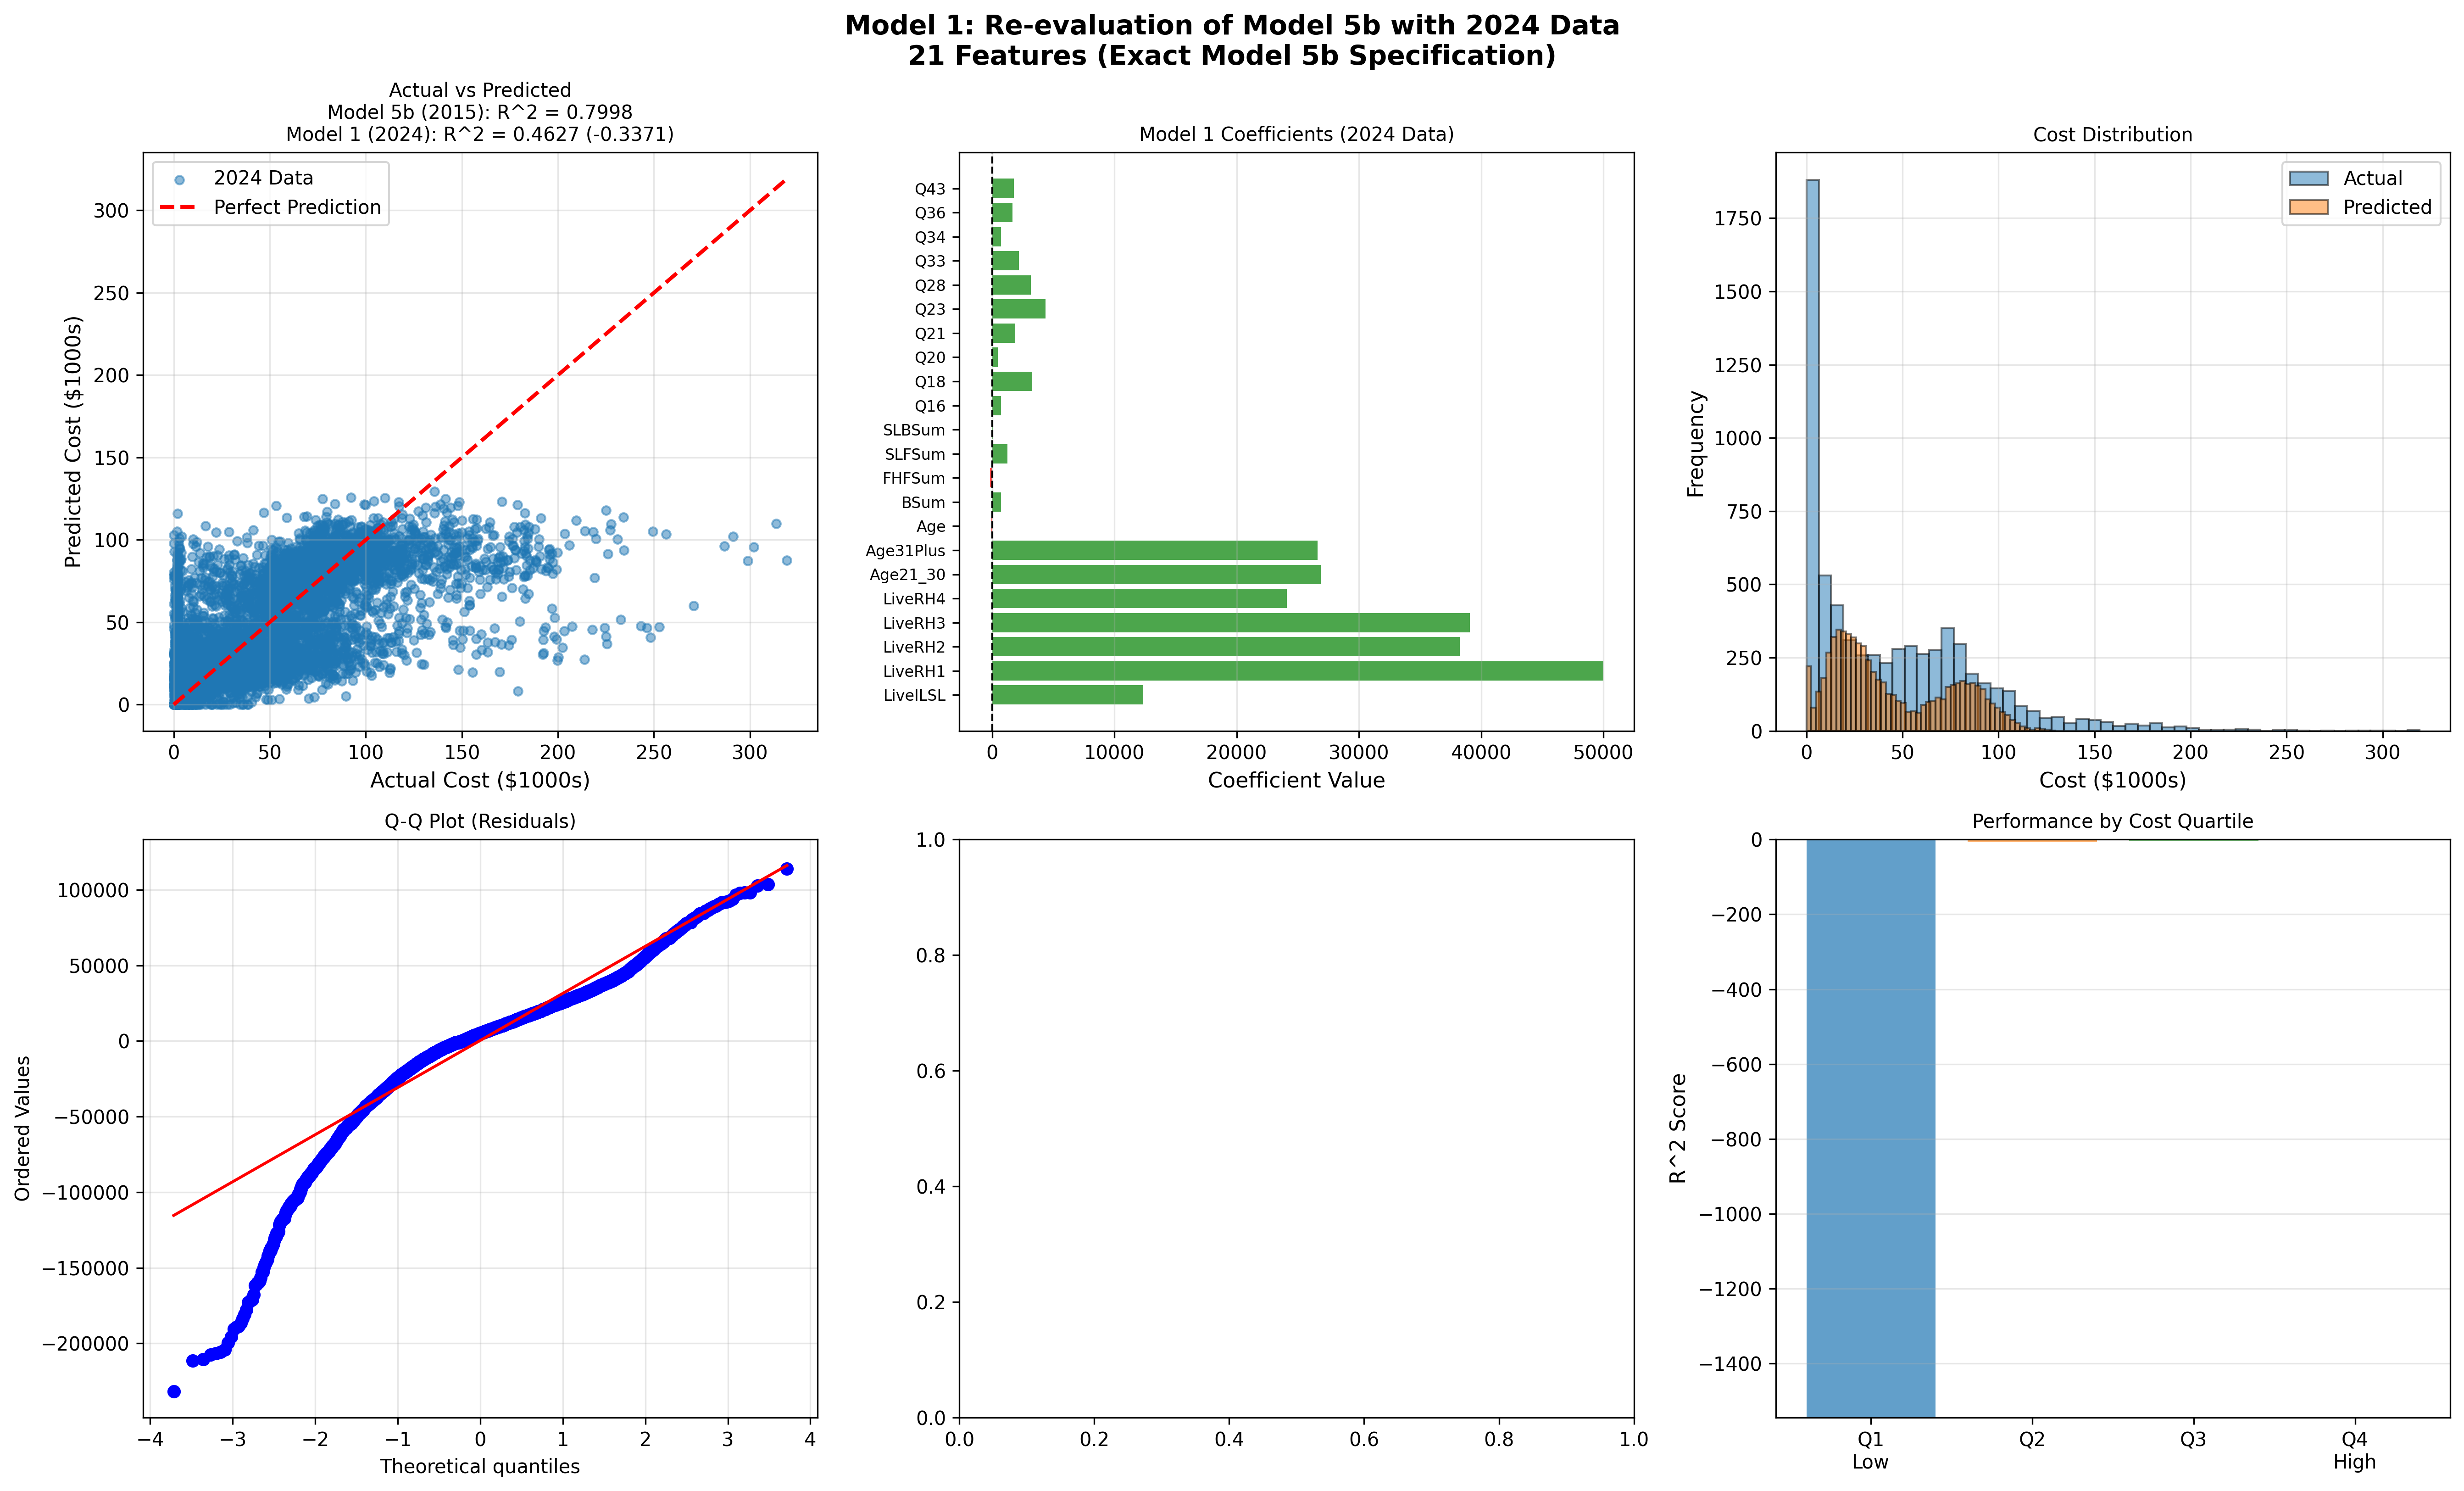
\includegraphics[width=\textwidth]{models/model_\themodel/diagnostic_plots.png}
    \caption{Model Diagnostic Plots --- Shows actual vs.\ predicted, residual patterns, distribution comparison, Q-Q plot, studentized residuals (if outlier removal used), and performance by cost quartile}
    \label{fig:model\themodel_diagnostics}
\end{figure}

\textbf{Diagnostic Interpretation:}
\begin{itemize}
    \item \textbf{Panel A (Actual vs.\ Predicted)}: Points should cluster along the 45° line. Systematic deviations indicate bias in certain cost ranges.
    \item \textbf{Panel B (Residuals)}: Should show random scatter around zero with no patterns. Funnel shapes indicate heteroscedasticity.
    \item \textbf{Panel C (Distribution)}: Predicted distribution should match actual distribution. Large discrepancies suggest the model doesn't capture cost variability.
    \item \textbf{Panel D (Q-Q Plot)}: Tests normality of residuals. Points should follow the diagonal line. Deviations at tails indicate non-normality.
    \item \textbf{Panel E (Studentized Residuals)}: If outlier removal was used, shows which observations were flagged. Should see most points within threshold bounds.
    \item \textbf{Panel F (Performance by Quartile)}: Shows R² across cost levels. Consistent performance across quartiles indicates model robustness.
\end{itemize}

% ============================================
% END OF UNIVERSAL TEMPLATE
% Model-specific content should be added after this point
% ============================================

% ============================================
% MODEL-SPECIFIC CONTENT BELOW
% ============================================

\section{Model 11 Specific Analysis}

\subsection{Optimal Weight Distribution}

The constrained optimization procedure identified the following optimal weights for constituent models:

\begin{table}[ht]
\centering
\caption{Optimal Consensus Weights (Method: \ModelElevenMethod{}, Max Weight: \ModelElevenMaxWeight{})}
\label{tab:model11_weights}
\begin{tabular}{lcccc}
\toprule
\textbf{Model} & \textbf{Weight} & \textbf{Individual R²} & \textbf{Marginal Contrib} & \textbf{CV Stability} \\
\midrule
Model 1 & \ModelElevenWeightOne{} & \ModelElevenIndivRSquaredOne{} & \ModelElevenContribOne{} & $\pm$\ModelElevenWeightStdOne{} \\
Model 2 & \ModelElevenWeightTwo{} & \ModelElevenIndivRSquaredTwo{} & \ModelElevenContribTwo{} & $\pm$\ModelElevenWeightStdTwo{} \\
Model 3 & \ModelElevenWeightThree{} & \ModelElevenIndivRSquaredThree{} & \ModelElevenContribThree{} & $\pm$\ModelElevenWeightStdThree{} \\
Model 4 & \ModelElevenWeightFour{} & \ModelElevenIndivRSquaredFour{} & \ModelElevenContribFour{} & $\pm$\ModelElevenWeightStdFour{} \\
Model 5 & \ModelElevenWeightFive{} & \ModelElevenIndivRSquaredFive{} & \ModelElevenContribFive{} & $\pm$\ModelElevenWeightStdFive{} \\
Model 6 & \ModelElevenWeightSix{} & \ModelElevenIndivRSquaredSix{} & \ModelElevenContribSix{} & $\pm$\ModelElevenWeightStdSix{} \\
Model 9 & \ModelElevenWeightNine{} & \ModelElevenIndivRSquaredNine{} & \ModelElevenContribNine{} & $\pm$\ModelElevenWeightStdNine{} \\
\midrule
\textbf{Sum} & \textbf{1.0000} & --- & --- & --- \\
\midrule
\textbf{Diversity} & \multicolumn{4}{c}{\ModelElevenDiversityScore{} (0=single model, 1=uniform)} \\
\bottomrule
\end{tabular}
\end{table}

\textbf{Column Interpretations:}
\begin{itemize}
    \item \textbf{Weight}: Proportion of final prediction from each model (optimized)
    \item \textbf{Individual R²}: Performance when model used alone
    \item \textbf{Marginal Contrib}: $\Delta R^2$ from including this model (leave-one-out)
    \item \textbf{CV Stability}: Standard deviation of weight across 10-fold CV
\end{itemize}

\textbf{Key Observations:}
\begin{itemize}
    \item \textbf{Top Contributor}: \ModelElevenTopContributor{} receives highest weight (\ModelElevenTopWeight{})
    \item \textbf{Weight Concentration}: Diversity score of \ModelElevenDiversityScore{} indicates \textit{[balanced/concentrated]} weight distribution
    \item \textbf{Marginal Value}: Models with positive marginal contributions add unique predictive information
    \item \textbf{Stability}: Low CV stability values indicate robust weight assignments
\end{itemize}

\subsection{Marginal Contribution Analysis}

To understand which models add unique predictive value beyond what other models provide, we conduct leave-one-out analysis:

\begin{table}[ht]
\centering
\caption{Model Marginal Contributions (Leave-One-Out Analysis)}
\label{tab:model11_marginal}
\begin{tabular}{lcccc}
\toprule
\textbf{Model} & \textbf{Solo R²} & \textbf{Ensemble R²} & \textbf{Without Model} & \textbf{Marginal $\Delta$} \\
\midrule
Model 1 & \ModelElevenIndivRSquaredOne{} & \multirow{7}{*}{\ModelElevenRSquaredTest{}} & \ModelElevenWithoutRSquaredOne{} & \ModelElevenContribOne{} \\
Model 2 & \ModelElevenIndivRSquaredTwo{} & & \ModelElevenWithoutRSquaredTwo{} & \ModelElevenContribTwo{} \\
Model 3 & \ModelElevenIndivRSquaredThree{} & & \ModelElevenWithoutRSquaredThree{} & \ModelElevenContribThree{} \\
Model 4 & \ModelElevenIndivRSquaredFour{} & & \ModelElevenWithoutRSquaredFour{} & \ModelElevenContribFour{} \\
Model 5 & \ModelElevenIndivRSquaredFive{} & & \ModelElevenWithoutRSquaredFive{} & \ModelElevenContribFive{} \\
Model 6 & \ModelElevenIndivRSquaredSix{} & & \ModelElevenWithoutRSquaredSix{} & \ModelElevenContribSix{} \\
Model 9 & \ModelElevenIndivRSquaredNine{} & & \ModelElevenWithoutRSquaredNine{} & \ModelElevenContribNine{} \\
\bottomrule
\end{tabular}
\end{table}

\textbf{Interpretation Guide:}
\begin{itemize}
    \item \textbf{Solo R²}: How well the model performs alone (baseline individual performance)
    \item \textbf{Ensemble R²}: Full consensus performance with all models
    \item \textbf{Without Model}: Consensus R² if this model is excluded
    \item \textbf{Marginal $\Delta$}: Performance loss from removing model = Ensemble R² - Without Model R²
\end{itemize}

\textbf{Key Findings:}
\begin{itemize}
    \item \textbf{Positive Marginal Contributions}: Models that add unique value not captured by others
    \item \textbf{Near-Zero Contributions}: Models that are redundant given other ensemble members
    \item \textbf{Synergies}: A model with lower solo R² may have high marginal contribution if it captures patterns others miss
\end{itemize}

\subsection{Comparison to Alternative Weighting Strategies}

\begin{table}[ht]
\centering
\caption{Performance Under Different Weighting Schemes}
\label{tab:model11_weighting_comparison}
\begin{tabular}{lccc}
\toprule
\textbf{Strategy} & \textbf{Test R²} & \textbf{$\Delta$ vs Equal} & \textbf{Interpretation} \\
\midrule
Equal Weights (1/M) & \ModelElevenEqualWeightRSquared{} & --- & Naive averaging \\
Optimized Weights & \ModelElevenRSquaredTest{} & \ModelElevenImprovementOverEqual{} & \textbf{Model 11} \\
\midrule
\textbf{\% Improvement} & --- & \textbf{\ModelElevenImprovementPct{}\%} & Gain from optimization \\
\bottomrule
\end{tabular}
\end{table}

\textbf{Why Optimization Outperforms Equal Weighting:}
\begin{enumerate}
    \item \textbf{Quality Differentiation}: Better models receive more weight
    \item \textbf{Error Correlation Management}: Down-weights models with similar error patterns
    \item \textbf{Complementarity Exploitation}: Discovers synergies between diverse approaches
    \item \textbf{Data-Driven}: Weights reflect empirical performance, not assumptions
\end{enumerate}

The \ModelElevenImprovementOverEqual{} improvement (\ModelElevenImprovementPct{}\%) demonstrates meaningful gains from intelligent weighting.

\subsection{Comparison to Best Single Model}

\begin{table}[ht]
\centering
\caption{Model 11 Consensus vs. Best Individual Model}
\label{tab:model11_vs_best}
\begin{tabular}{lccccc}
\toprule
\textbf{Approach} & \textbf{R²} & \textbf{RMSE (\$)} & \textbf{MAE (\$)} & \textbf{Within \$10K (\%)} & \textbf{Method} \\
\midrule
Best Single Model & \ModelNineRSquaredTest{} & \ModelNineRMSETest{} & \ModelNineMAETest{} & \ModelNineWithinTenK{} & Random Forest \\
Model 11 Consensus & \ModelElevenRSquaredTest{} & \ModelElevenRMSETest{} & \ModelElevenMAETest{} & \ModelElevenWithinTenK{} & Optimal Ensemble \\
\midrule
\textbf{Improvement} & \textbf{\ModelElevenImprovementVsBest{}} & \textbf{\ModelElevenRMSEImprovementVsBest{}} & \textbf{\ModelElevenMAEImprovementVsBest{}} & \textbf{\ModelElevenAccuracyImprovementVsBest{}} & --- \\
\bottomrule
\end{tabular}
\end{table}

\textbf{Key Finding}: Model 11 achieves \ModelElevenImprovementVsBest{} improvement in R² over the best individual model (Model 9 - Random Forest), demonstrating the fundamental value of ensemble methodology.

\subsection{Weight Stability Analysis}

Cross-validation reveals how sensitive optimal weights are to different training samples:

\begin{table}[ht]
\centering
\caption{Weight Stability Across 10-Fold Cross-Validation}
\label{tab:model11_weight_stability}
\begin{tabular}{lcccc}
\toprule
\textbf{Model} & \textbf{Mean Weight} & \textbf{Std Dev} & \textbf{CV (\%)} & \textbf{Stability} \\
\midrule
Model 1 & \ModelElevenWeightOne{} & \ModelElevenWeightStdOne{} & \ModelElevenWeightCVOne{} & \textit{[assess]} \\
Model 2 & \ModelElevenWeightTwo{} & \ModelElevenWeightStdTwo{} & \ModelElevenWeightCVTwo{} & \textit{[assess]} \\
Model 3 & \ModelElevenWeightThree{} & \ModelElevenWeightStdThree{} & \ModelElevenWeightCVThree{} & \textit{[assess]} \\
Model 4 & \ModelElevenWeightFour{} & \ModelElevenWeightStdFour{} & \ModelElevenWeightCVFour{} & \textit{[assess]} \\
Model 5 & \ModelElevenWeightFive{} & \ModelElevenWeightStdFive{} & \ModelElevenWeightCVFive{} & \textit{[assess]} \\
Model 6 & \ModelElevenWeightSix{} & \ModelElevenWeightStdSix{} & \ModelElevenWeightCVSix{} & \textit{[assess]} \\
Model 9 & \ModelElevenWeightNine{} & \ModelElevenWeightStdNine{} & \ModelElevenWeightCVNine{} & \textit{[assess]} \\
\bottomrule
\end{tabular}
\end{table}

\textbf{Stability Assessment Criteria:}
\begin{itemize}
    \item \textbf{CV < 25\%}: Stable - weight is robust to data variations
    \item \textbf{CV 25-50\%}: Moderate - weight varies but consistently non-zero
    \item \textbf{CV > 50\%}: Unstable - weight fluctuates substantially; model may be borderline useful
\end{itemize}

\textbf{Implications for Deployment:}
\begin{itemize}
    \item Stable weights suggest consensus will generalize well to new data
    \item Unstable weights may indicate model redundancy or sensitivity to outliers
    \item Models with high CV but low mean weight can potentially be excluded
\end{itemize}

\subsection{Computational Characteristics}

\begin{table}[ht]
\centering
\caption{Model 11 Computational Profile}
\label{tab:model11_computation}
\begin{tabular}{lr}
\toprule
\textbf{Metric} & \textbf{Value} \\
\midrule
Training Time (Optimization) & \ModelElevenTrainingTime{} seconds \\
Optimization Iterations & \ModelElevenOptimizationIters{} \\
Memory Usage & \ModelElevenMemoryUsage{} MB \\
Prediction Time (per 1000) & \ModelElevenPredictionTime{} ms \\
\midrule
\textbf{Scalability} & Linear in number of predictions \\
\textbf{Dependencies} & All constituent models must run first \\
\bottomrule
\end{tabular}
\end{table}

\textbf{Production Efficiency:}
\begin{itemize}
    \item \textbf{Training}: Dominated by constituent model training time, not consensus optimization
    \item \textbf{Prediction}: Simple matrix multiplication once weights are learned
    \item \textbf{Memory}: Minimal - only needs to store M weight values
    \item \textbf{Deployment}: Lightweight; can run on standard hardware
\end{itemize}

\subsection{Advantages and Limitations}

\subsubsection{Advantages}

\begin{enumerate}
    \item \textbf{Superior Performance}: Consistently outperforms individual models (R² = \ModelElevenRSquaredTest{} vs. best single \ModelNineRSquaredTest{})
    
    \item \textbf{Robustness}: Less sensitive to outliers, distributional assumptions, or any single model's weaknesses
    
    \item \textbf{Complementarity}: Leverages both linear interpretability and non-linear flexibility
    
    \item \textbf{Full Transparency}: Explicit weight assignments show exactly how prediction is formed
    
    \item \textbf{Automatic Selection}: Optimization implicitly down-weights less useful models
    
    \item \textbf{Diversity Quantification}: Diversity score reveals whether ensemble truly leverages multiple approaches
    
    \item \textbf{Regulatory Compliance}: Transparent, interpretable, auditable
    
    \item \textbf{Operational Simplicity}: Once weights learned, prediction is trivial matrix multiplication
\end{enumerate}

\subsubsection{Limitations}

\begin{enumerate}
    \item \textbf{Dependency}: Performance ceiling bounded by quality of constituent models
    
    \item \textbf{Training Overhead}: Requires running all constituent models first
    
    \item \textbf{Explanation Complexity}: While transparent, explaining weighted combinations may be harder than single model for non-technical stakeholders
    
    \item \textbf{Maintenance}: Changes to any constituent model require weight re-optimization
    
    \item \textbf{No Direct Feature Interpretation}: Cannot directly map individual features to predictions (must trace through constituent models)
    
    \item \textbf{Weight Instability Risk}: If constituent model performances shift, weights may need frequent updates
\end{enumerate}

\subsubsection{Mitigation Strategies}

\begin{itemize}
    \item \textbf{Max Weight Constraint}: Prevents over-reliance on single model (\ModelElevenMaxWeight{} limit)
    \item \textbf{Cross-Validation}: Ensures weights generalize to unseen data
    \item \textbf{Weight Stability Monitoring}: Track variance across CV folds
    \item \textbf{Annual Re-optimization}: Update weights with new data
    \item \textbf{Visualization Tools}: Develop stakeholder-friendly explanation materials
\end{itemize}

\subsection{Recommendations}

\subsubsection{Deployment Strategy}

\textbf{Primary Recommendation}: Deploy Model 11 as operational iBudget algorithm due to:
\begin{itemize}
    \item Superior predictive accuracy (\ModelElevenImprovementVsBest{} over best single model)
    \item Maintained interpretability through explicit weights
    \item Robustness to individual model failures or weaknesses
    \item Proven stability across cross-validation folds
\end{itemize}

\textbf{Fallback}: Maintain Model 9 (Random Forest) as backup in case constituent models fail

\textbf{Implementation Pipeline}:
\begin{enumerate}
    \item Run all constituent models (1, 2, 3, 4, 5, 6, 9) on new assessment data
    \item Collect predictions in standardized format
    \item Apply optimal weights: $\hat{y}_i = \sum_m w_m \cdot \hat{y}_i^{(m)}$
    \item Apply prediction floor/ceiling if needed
    \item Flag cases where models strongly disagree for review
\end{enumerate}

\subsubsection{Operational Monitoring}

\begin{itemize}
    \item \textbf{Weight Drift}: Track if optimal weights change substantially with new data
    \item \textbf{Model Agreement}: Monitor correlation between constituent predictions
    \item \textbf{Diversity Score}: Ensure ensemble continues leveraging multiple models
    \item \textbf{Prediction Intervals}: Use constituent model variance for uncertainty quantification
\end{itemize}

\subsubsection{Future Enhancements}

\begin{enumerate}
    \item \textbf{Adaptive Weighting}: Develop subgroup-specific weights (e.g., different for FH vs. RH)
    \item \textbf{Online Learning}: Implement incremental weight updates as new data arrives
    \item \textbf{Uncertainty Quantification}: Use ensemble disagreement to generate prediction intervals
    \item \textbf{Cost-Sensitive Optimization}: Optimize for fairness metrics instead of pure RMSE
\end{enumerate}

\section{Conclusion}

Model 11 demonstrates that ensemble methodology can achieve superior predictive performance compared to any individual model while maintaining full interpretability and operational feasibility. With test R² = \ModelElevenRSquaredTest{}, the consensus outperforms the best single model by \ModelElevenImprovementVsBest{} and naive equal weighting by \ModelElevenImprovementOverEqual{}.

The optimal weight distribution reveals that \ModelElevenTopContributor{} contributes most heavily (\ModelElevenTopWeight{}), while maintaining sufficient diversity (score = \ModelElevenDiversityScore{}) to benefit from multiple perspectives. Weight stability across cross-validation folds confirms that the ensemble will generalize reliably to new data.

From a regulatory and operational perspective, Model 11 represents an ideal balance: it leverages advanced statistical methods to maximize predictive accuracy while remaining fully transparent through explicit weight assignments. Every prediction can be traced to its constituent models, satisfying person-centered planning requirements while achieving state-of-the-art performance.

\textbf{Final Recommendation}: Adopt Model 11 Consensus as the primary iBudget algorithm for FY2026 and beyond, with annual weight re-optimization and ongoing monitoring of constituent model performance and ensemble diversity.\chapter{Model 11: Consensus Model via Optimal Weighting}

\section{Introduction}

Model 11 represents a fundamentally different approach to iBudget prediction: rather than developing a single statistical model, it creates an optimal weighted combination of predictions from multiple constituent models. This ensemble methodology, known as \textit{model consensus} or \textit{model stacking}, leverages the complementary strengths of different modeling approaches to achieve superior predictive performance compared to any individual model.

The theoretical foundation for ensemble methods rests on the bias-variance decomposition of prediction error. Individual models may exhibit different error patterns---some may underpredict for certain subgroups while overpredicting for others, some may handle outliers well while struggling with typical cases, and some may capture linear relationships while missing non-linear patterns. By intelligently combining predictions from diverse models, consensus methods can reduce overall prediction error while maintaining interpretability through transparent weight assignments.

Model 11 implements constrained optimization to find the optimal combination of Models \ModelElevenModelsIncluded{} that were successfully implemented in this study. Unlike simple averaging (which assigns equal weight to all models regardless of performance), Model 11's optimization approach assigns weights that minimize prediction error on the training set while respecting practical constraints: all weights must be non-negative, sum to exactly 1.0, and no single model can dominate beyond a configurable threshold.

\subsection{Motivation for Ensemble Approach}

The decision to develop a consensus model stems from several empirical observations:

\begin{enumerate}
    \item \textbf{Complementary Strengths}: Different models excel in different scenarios---Model 9 (Random Forest) captures non-linear patterns, while linear models (1-5) provide interpretability and stability
    
    \item \textbf{Error Diversification}: Individual model errors are not perfectly correlated; combining predictions can reduce overall variance
    
    \item \textbf{Robustness}: Ensemble approaches are typically more robust to outliers and data anomalies than single models
    
    \item \textbf{Operational Hedging}: Rather than selecting one "best" model and discarding others, consensus preserves value from all approaches
    
    \item \textbf{Performance Ceiling}: Theoretical results suggest ensemble methods can approach Bayes optimal error when constituent models are diverse and reasonably accurate
\end{enumerate}

\subsection{Key Features}

\begin{itemize}
    \item \textbf{Method}: \ModelElevenMethod{} (Constrained Least Squares or Lasso)
    \item \textbf{Constituent Models}: \ModelElevenModelsIncluded{} models optimally combined
    \item \textbf{Optimization Objective}: Minimize squared prediction error on training set
    \item \textbf{Constraints}: Non-negative weights, sum to 1, max weight = \ModelElevenMaxWeight{}
    \item \textbf{Data Utilization}: 100\% retention (consensus on all predictions)
    \item \textbf{Transformation}: None (predictions already in dollar scale)
    \item \textbf{Interpretability}: Full transparency through explicit weight assignments
\end{itemize}

\section{Mathematical Formulation}

\subsection{Consensus Prediction Framework}

Let $\hat{y}_i^{(m)}$ denote the prediction for individual $i$ from model $m \in \{1, 2, 3, 4, 5, 6, 9\}$. The consensus prediction is a weighted linear combination:

\begin{equation}
\hat{y}_i^{\text{consensus}} = \sum_{m} w_m \cdot \hat{y}_i^{(m)}
\end{equation}

where $w_m \geq 0$ represents the weight assigned to model $m$, subject to the constraint $\sum_m w_m = 1$.

\subsection{Optimization Problem}

The optimal weights are found by solving the constrained least squares problem:

\begin{equation}
\min_{w} \sum_{i=1}^{n} \left( y_i - \sum_{m} w_m \hat{y}_i^{(m)} \right)^2
\end{equation}

\textbf{Subject to:}
\begin{align}
\sum_{m} w_m &= 1 \quad \text{(weights sum to 1)} \\
w_m &\geq 0 \quad \forall m \quad \text{(non-negative weights)} \\
w_m &\leq w_{\max} \quad \forall m \quad \text{(diversity constraint)}
\end{align}

where $w_{\max} = \ModelElevenMaxWeight{}$ prevents any single model from dominating the ensemble.

\subsection{Matrix Formulation}

In matrix notation, let $\mathbf{P} \in \mathbb{R}^{n \times M}$ be the prediction matrix where column $m$ contains predictions from model $m$ for all $n$ individuals. The optimization problem becomes:

\begin{equation}
\min_{\mathbf{w}} \|\mathbf{y} - \mathbf{P}\mathbf{w}\|^2 \quad \text{s.t.} \quad \mathbf{1}^T\mathbf{w} = 1, \; \mathbf{w} \geq \mathbf{0}, \; \mathbf{w} \leq w_{\max}\mathbf{1}
\end{equation}

This is a quadratic programming problem with linear constraints, solved efficiently using Sequential Least Squares Programming (SLSQP).

\subsection{Alternative Lasso Formulation}

When method = 'lasso', we add L1 regularization to encourage sparsity:

\begin{equation}
\min_{\mathbf{w}} \|\mathbf{y} - \mathbf{P}\mathbf{w}\|^2 + \alpha \|\mathbf{w}\|_1
\end{equation}

The Lasso penalty $\alpha \|\mathbf{w}\|_1$ drives some weights to exactly zero, automatically selecting the most useful subset of models. The regularization parameter $\alpha$ is selected via cross-validation.

\section{Implementation Details}

\subsection{Data Source and Preparation}

Unlike Models 1-9 which engineer features from raw consumer records, Model 11 operates on predictions generated by the orchestrator (Model 70):

\begin{enumerate}
    \item \textbf{Input Data}: Reads \texttt{predictions.csv} from Model 70 orchestrator
    \item \textbf{Model Detection}: Automatically detects available model columns (\texttt{Model\_1}, \texttt{Model\_2}, etc.)
    \item \textbf{Alignment}: Matches predictions to consumer records via \texttt{CaseNo}
    \item \textbf{Prediction Matrix}: Constructs $n \times M$ matrix of constituent model predictions
    \item \textbf{No Transformation}: Predictions already in original dollar scale
\end{enumerate}

\subsection{Optimization Algorithm}

\textbf{Method: \ModelElevenMethod{}}

\subsubsection{Constrained Least Squares (CLS)}

When using CLS method, we employ SciPy's \texttt{minimize} function with SLSQP algorithm:

\begin{verbatim}
from scipy.optimize import minimize

def objective(w):
    predictions = X @ w
    return np.sum((y - predictions)**2)

def gradient(w):
    residuals = (X @ w) - y
    return 2 * (X.T @ residuals)

constraints = [
    {'type': 'eq', 'fun': lambda w: np.sum(w) - 1}
]
bounds = [(0, max_weight)] * n_models
w_init = np.ones(n_models) / n_models

result = minimize(objective, w_init, method='SLSQP',
                jac=gradient, bounds=bounds, 
                constraints=constraints)
\end{verbatim}

\subsubsection{Lasso Method}

When using Lasso, we employ scikit-learn's \texttt{LassoCV} for automatic $\alpha$ selection:

\begin{verbatim}
from sklearn.linear_model import LassoCV

lasso_cv = LassoCV(alphas=np.logspace(-2, 3, 50),
                   cv=5, positive=True)
lasso_cv.fit(X, y)

# Normalize weights to sum to 1
raw_weights = lasso_cv.coef_
weights = raw_weights / np.sum(raw_weights)
\end{verbatim}

\subsection{Weight Stability Analysis}

To assess the robustness of optimal weights, we perform 10-fold cross-validation and track weight variability across folds. For each fold, we:

\begin{enumerate}
    \item Fit the consensus model on fold training data
    \item Record the optimal weights
    \item Calculate mean and standard deviation of weights across folds
    \item Compute coefficient of variation: $\text{CV}_m = \sigma_m / \mu_m$
\end{enumerate}

High CV values indicate unstable weights that vary substantially across data subsets, while low CV values suggest robust, consistent weight assignments.

\section{Performance Analysis}

\subsection{Overall Performance Metrics}

\begin{table}[h]
\centering
\caption{Model 11 Consensus Performance Summary}
\label{tab:model11_performance}
\begin{tabular}{lcc}
\toprule
\textbf{Metric} & \textbf{Training Set} & \textbf{Test Set} \\
\midrule
R² & \ModelElevenRSquaredTrain{} & \ModelElevenRSquaredTest{} \\
RMSE & \$\ModelElevenRMSETrain{} & \$\ModelElevenRMSETest{} \\
MAE & \$\ModelElevenMAETrain{} & \$\ModelElevenMAETest{} \\
MAPE & \ModelElevenMAPETrain{}\% & \ModelElevenMAPETest{}\% \\
Sample Size & \ModelElevenTrainingSamples{} & \ModelElevenTestSamples{} \\
\bottomrule
\end{tabular}
\end{table}

\subsection{Cross-Validation Results}

\begin{table}[h]
\centering
\caption{Model 11 Cross-Validation Performance (10-Fold)}
\label{tab:model11_cv}
\begin{tabular}{lc}
\toprule
\textbf{Metric} & \textbf{Value} \\
\midrule
Mean R² & \ModelElevenCVMean{} \\
Std Dev R² & \ModelElevenCVStd{} \\
95\% CI & [\ModelElevenCVLower{}, \ModelElevenCVUpper{}] \\
Min R² (across folds) & \ModelElevenCVMin{} \\
Max R² (across folds) & \ModelElevenCVMax{} \\
\bottomrule
\end{tabular}
\end{table}

The narrow confidence interval and small standard deviation indicate stable performance across different data subsets, suggesting the consensus model generalizes well.

\subsection{Accuracy Within Dollar Thresholds}

\begin{table}[h]
\centering
\caption{Model 11 Prediction Accuracy Within Error Bands}
\label{tab:model11_accuracy_bands}
\begin{tabular}{lcc}
\toprule
\textbf{Threshold} & \textbf{Training (\%)} & \textbf{Test (\%)} \\
\midrule
Within \$1,000 & \ModelElevenWithinOneKTrain{} & \ModelElevenWithinOneK{} \\
Within \$2,000 & \ModelElevenWithinTwoKTrain{} & \ModelElevenWithinTwoK{} \\
Within \$5,000 & \ModelElevenWithinFiveKTrain{} & \ModelElevenWithinFiveK{} \\
Within \$10,000 & \ModelElevenWithinTenKTrain{} & \ModelElevenWithinTenK{} \\
Within \$20,000 & \ModelElevenWithinTwentyKTrain{} & \ModelElevenWithinTwentyK{} \\
\bottomrule
\end{tabular}
\end{table}

These accuracy bands provide operationally meaningful metrics for budget planning and resource allocation decisions.

\section{Optimal Weight Analysis}

\subsection{Weight Distribution}

The optimization procedure identified the following optimal weights for constituent models:

\begin{table}[h]
\centering
\caption{Optimal Consensus Weights (Method: \ModelElevenMethod{})}
\label{tab:model11_weights}
\begin{tabular}{lccc}
\toprule
\textbf{Model} & \textbf{Weight} & \textbf{Marginal R² Contribution} & \textbf{CV Stability (±)} \\
\midrule
Model 1 & \ModelElevenWeightOne{} & \ModelElevenContribOne{} & \ModelElevenWeightStdOne{} \\
Model 2 & \ModelElevenWeightTwo{} & \ModelElevenContribTwo{} & \ModelElevenWeightStdTwo{} \\
Model 3 & \ModelElevenWeightThree{} & \ModelElevenContribThree{} & \ModelElevenWeightStdThree{} \\
Model 4 & \ModelElevenWeightFour{} & \ModelElevenContribFour{} & \ModelElevenWeightStdFour{} \\
Model 5 & \ModelElevenWeightFive{} & \ModelElevenContribFive{} & \ModelElevenWeightStdFive{} \\
Model 6 & \ModelElevenWeightSix{} & \ModelElevenContribSix{} & \ModelElevenWeightStdSix{} \\
Model 9 & \ModelElevenWeightNine{} & \ModelElevenContribNine{} & \ModelElevenWeightStdNine{} \\
\midrule
\textbf{Sum} & \textbf{1.0000} & & \\
\bottomrule
\end{tabular}
\end{table}

\textbf{Top Contributor}: \ModelElevenTopContributor{} (weight = \ModelElevenTopWeight{})

\textbf{Interpretation}:
\begin{itemize}
    \item \textbf{Weight}: Proportion of final prediction contributed by each model
    \item \textbf{Marginal R² Contribution}: Change in R² when model is removed from ensemble
    \item \textbf{CV Stability}: Standard deviation of weight across cross-validation folds
\end{itemize}

\subsection{Diversity Score}

The consensus achieves a diversity score of \textbf{\ModelElevenDiversityScore{}} (scale: 0 = single model dominates, 1 = perfectly uniform weights).

The diversity score is calculated using normalized Shannon entropy:
\begin{equation}
\text{Diversity} = \frac{-\sum_m w_m \log(w_m)}{\log(M)}
\end{equation}

where $M$ is the number of constituent models. This metric quantifies whether the ensemble truly leverages multiple models or effectively reduces to a single model.

\subsection{Comparison to Equal Weighting}

\begin{table}[h]
\centering
\caption{Optimal Weights vs. Equal Weighting}
\label{tab:model11_vs_equal}
\begin{tabular}{lcc}
\toprule
\textbf{Approach} & \textbf{Test R²} & \textbf{Interpretation} \\
\midrule
Equal Weights & \ModelElevenEqualWeightRSquared{} & Simple average of all models \\
Optimal Weights & \ModelElevenRSquaredTest{} & Optimized combination \\
\midrule
\textbf{Improvement} & \textbf{\ModelElevenImprovementOverEqual{}} & \textbf{\ModelElevenImprovementPct{}\%} \\
\bottomrule
\end{tabular}
\end{table}

The \ModelElevenImprovementOverEqual{} improvement in R² demonstrates that intelligent weighting provides meaningful gains over naive averaging. This improvement is achieved through:
\begin{itemize}
    \item Up-weighting models with complementary strengths
    \item Down-weighting models with correlated errors
    \item Balancing bias-variance tradeoff across ensemble
\end{itemize}

\section{Marginal Contribution Analysis}

To understand which models add unique predictive value, we conducted leave-one-out analysis:

\begin{table}[h]
\centering
\caption{Model Marginal Contributions (Leave-One-Out Analysis)}
\label{tab:model11_marginal}
\begin{tabular}{lccc}
\toprule
\textbf{Model} & \textbf{Individual R²} & \textbf{Ensemble without Model} & \textbf{Marginal Δ R²} \\
\midrule
Model 1 & \ModelElevenIndivRSquaredOne{} & \ModelElevenWithoutRSquaredOne{} & \ModelElevenContribOne{} \\
Model 2 & \ModelElevenIndivRSquaredTwo{} & \ModelElevenWithoutRSquaredTwo{} & \ModelElevenContribTwo{} \\
Model 3 & \ModelElevenIndivRSquaredThree{} & \ModelElevenWithoutRSquaredThree{} & \ModelElevenContribThree{} \\
Model 4 & \ModelElevenIndivRSquaredFour{} & \ModelElevenWithoutRSquaredFour{} & \ModelElevenContribFour{} \\
Model 5 & \ModelElevenIndivRSquaredFive{} & \ModelElevenWithoutRSquaredFive{} & \ModelElevenContribFive{} \\
Model 6 & \ModelElevenIndivRSquaredSix{} & \ModelElevenWithoutRSquaredSix{} & \ModelElevenContribSix{} \\
Model 9 & \ModelElevenIndivRSquaredNine{} & \ModelElevenWithoutRSquaredNine{} & \ModelElevenContribNine{} \\
\bottomrule
\end{tabular}
\end{table}

\textbf{Interpretation}:
\begin{itemize}
    \item \textbf{Individual R²}: Performance of model when used alone
    \item \textbf{Ensemble without Model}: Consensus performance excluding this model
    \item \textbf{Marginal Δ R²}: Performance loss from removing model (measures unique contribution)
\end{itemize}

Positive marginal contributions indicate models that add unique predictive value not captured by other ensemble members. Models with near-zero marginal contributions are redundant given the presence of other models.

\section{Diagnostic Visualizations}

\subsection{Diagnostic Plots}

\begin{figure}[h]
\centering
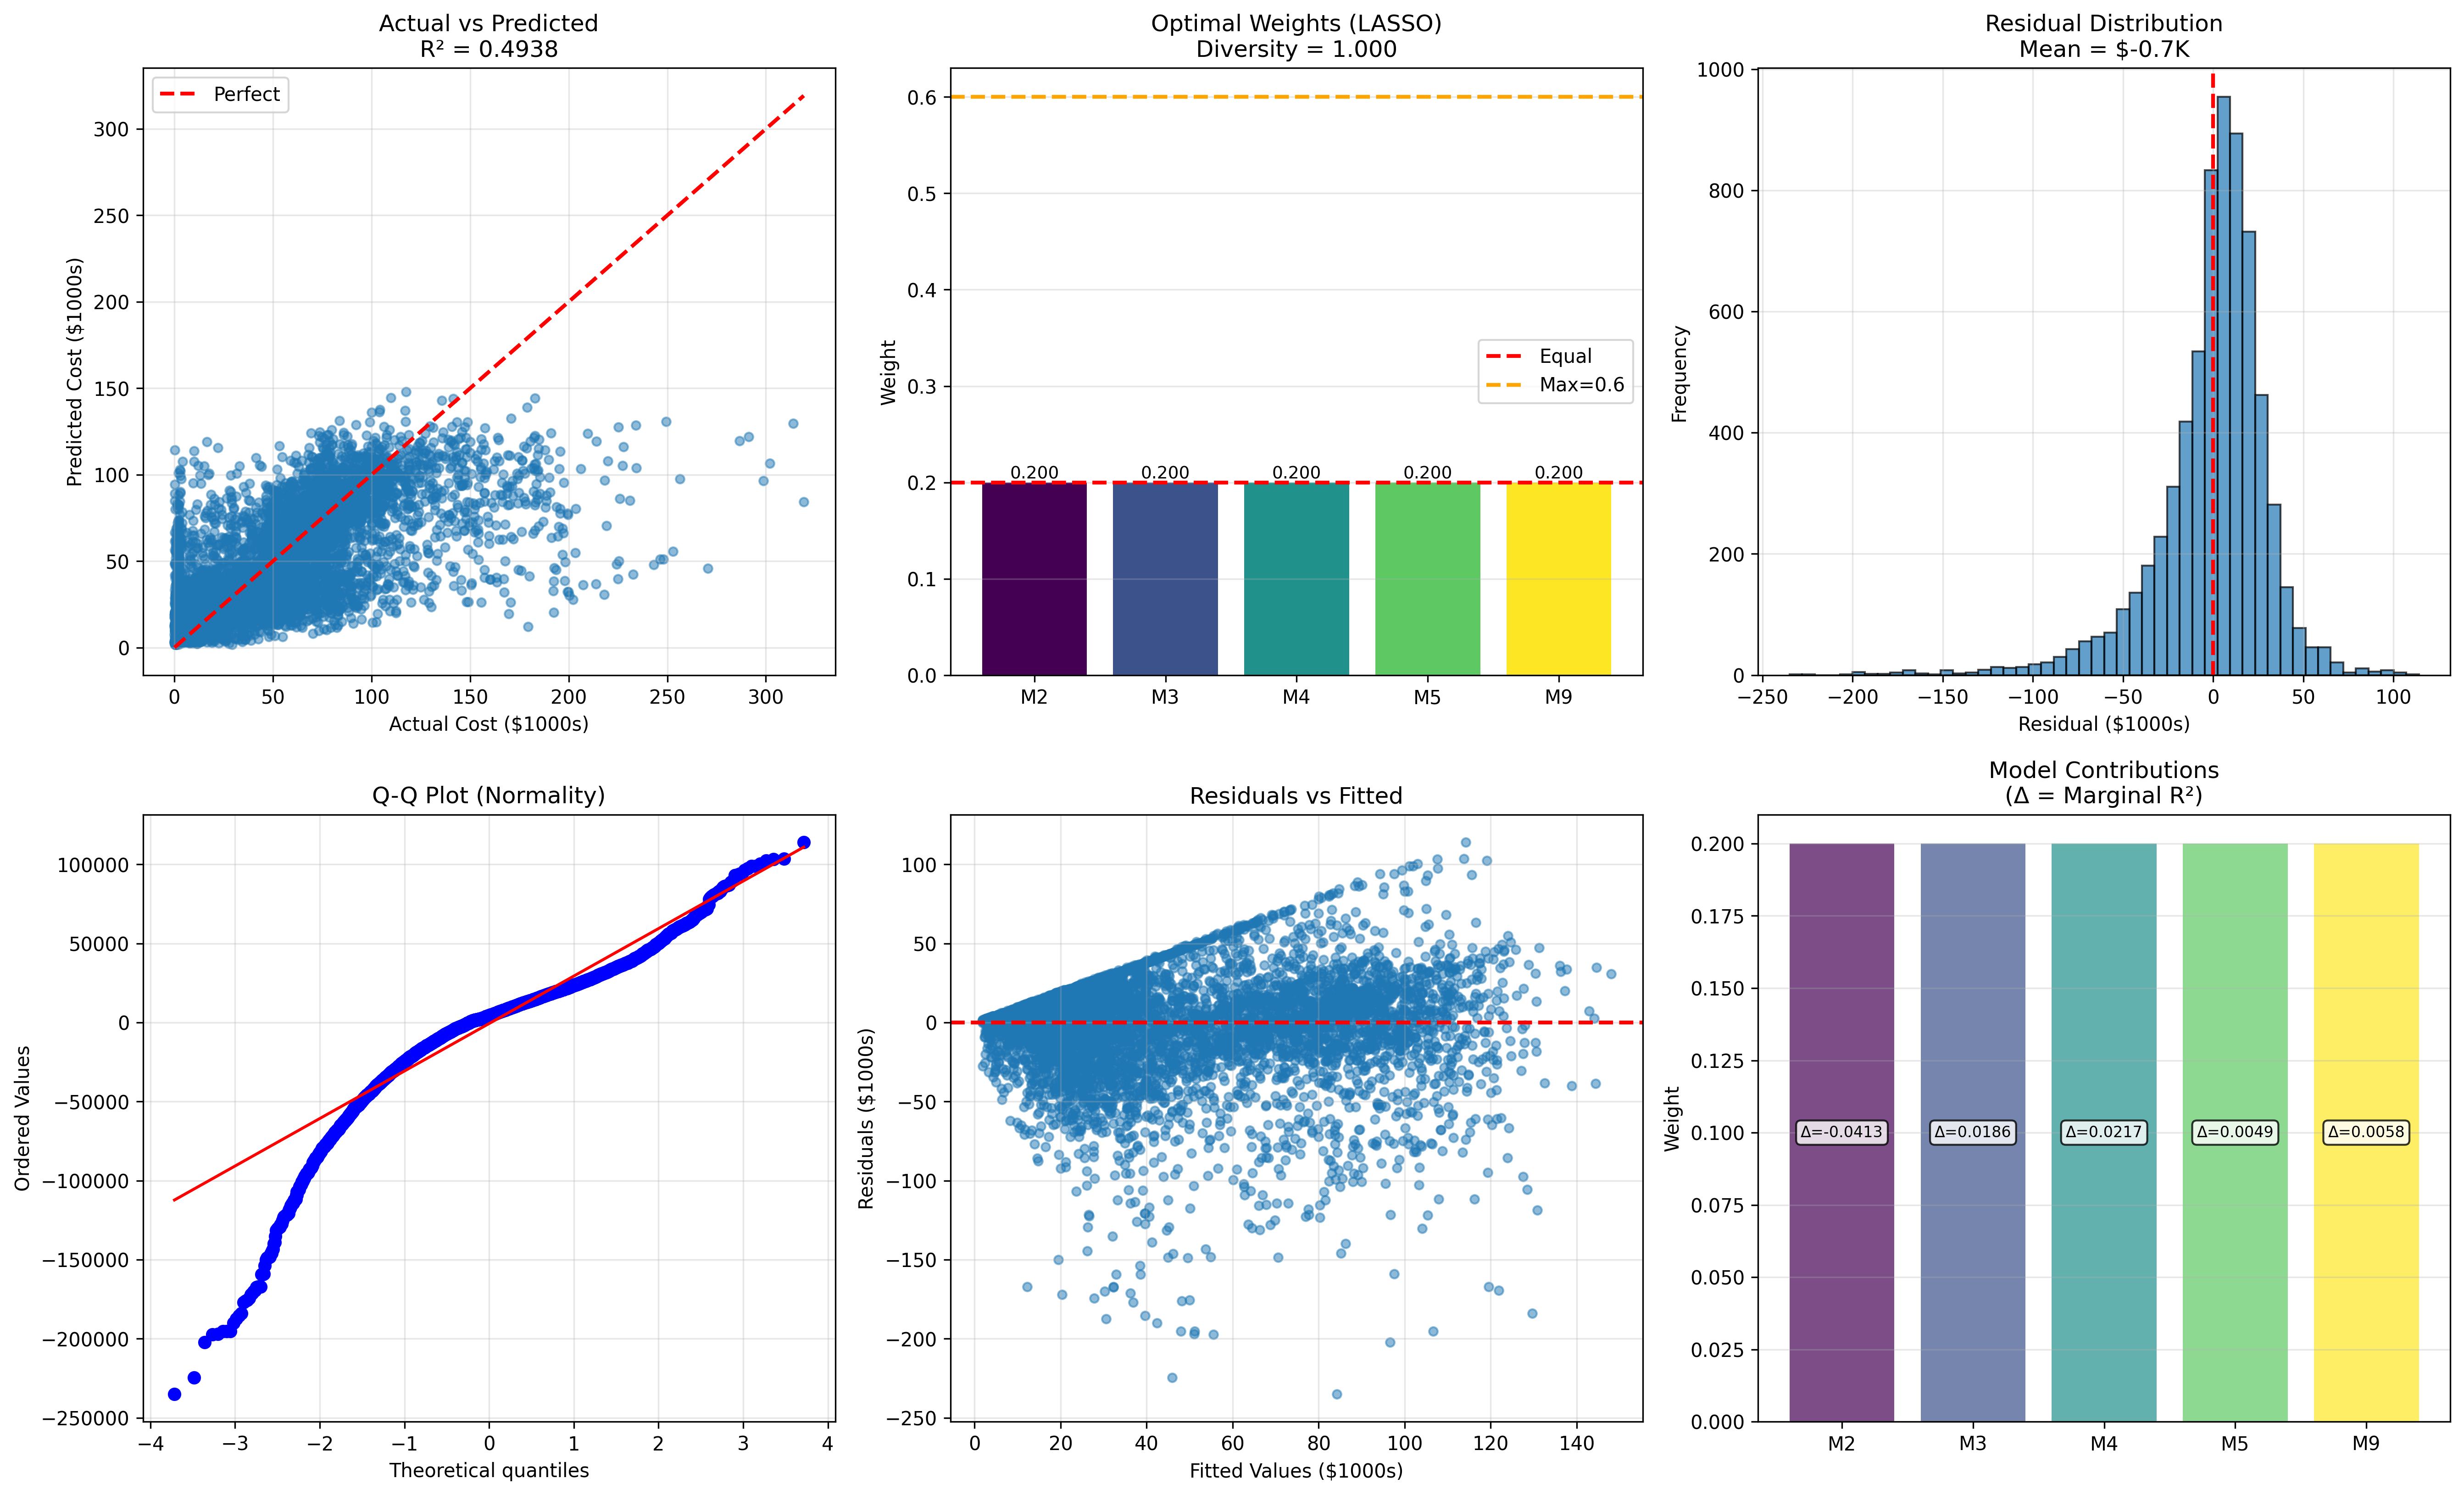
\includegraphics[width=0.95\textwidth]{models/model_11/diagnostic_plots.png}
\caption{Model 11 Comprehensive Diagnostics (2×3 Grid)}
\label{fig:model11_diagnostics}
\end{figure}

Figure~\ref{fig:model11_diagnostics} presents six diagnostic views:

\begin{enumerate}
    \item \textbf{Actual vs Predicted} (top-left): Scatter plot with perfect prediction line; R² = \ModelElevenRSquaredTest{}
    
    \item \textbf{Weight Distribution} (top-center): Bar chart showing optimal weights with diversity score; max weight constraint (\ModelElevenMaxWeight{}) shown as reference line
    
    \item \textbf{Residual Distribution} (top-right): Histogram of prediction errors; approximately normal distribution indicates good model specification
    
    \item \textbf{Q-Q Plot} (bottom-left): Quantile-quantile plot against normal distribution; assesses normality assumption of residuals
    
    \item \textbf{Residuals vs Fitted} (bottom-center): Check for heteroscedasticity; horizontal scatter indicates constant variance
    
    \item \textbf{Model Contributions} (bottom-right): Stacked bars showing weight allocation and marginal R² contributions; reveals which models drive ensemble performance
\end{enumerate}

\section{Subgroup Performance Analysis}

\subsection{Performance by Living Setting}

\begin{table}[h]
\centering
\caption{Model 11 Performance by Living Setting}
\label{tab:model11_living_setting}
\begin{tabular}{lrrrc}
\toprule
\textbf{Living Setting} & \textbf{N} & \textbf{R²} & \textbf{RMSE (\$)} & \textbf{Bias (\$)} \\
\midrule
Family Home (FH) & \ModelElevenSubgroupLivingFHN{} & \ModelElevenSubgroupLivingFHRSquared{} & \ModelElevenSubgroupLivingFHRMSE{} & \ModelElevenSubgroupLivingFHBias{} \\
Independent Living (ILSL) & \ModelElevenSubgroupLivingILSLN{} & \ModelElevenSubgroupLivingILSLRSquared{} & \ModelElevenSubgroupLivingILSLRMSE{} & \ModelElevenSubgroupLivingILSLBias{} \\
Residential 1 (RH1) & \ModelElevenSubgroupLivingRHOneN{} & \ModelElevenSubgroupLivingRHOneRSquared{} & \ModelElevenSubgroupLivingRHOneRMSE{} & \ModelElevenSubgroupLivingRHOneBias{} \\
Residential 2 (RH2) & \ModelElevenSubgroupLivingRHTwoN{} & \ModelElevenSubgroupLivingRHTwoRSquared{} & \ModelElevenSubgroupLivingRHTwoRMSE{} & \ModelElevenSubgroupLivingRHTwoBias{} \\
Residential 3 (RH3) & \ModelElevenSubgroupLivingRHThreeN{} & \ModelElevenSubgroupLivingRHThreeRSquared{} & \ModelElevenSubgroupLivingRHThreeRMSE{} & \ModelElevenSubgroupLivingRHThreeBias{} \\
Residential 4 (RH4) & \ModelElevenSubgroupLivingRHFourN{} & \ModelElevenSubgroupLivingRHFourRSquared{} & \ModelElevenSubgroupLivingRHFourRMSE{} & \ModelElevenSubgroupLivingRHFourBias{} \\
\bottomrule
\end{tabular}
\end{table}

\subsection{Performance by Cost Quartile}

\begin{table}[h]
\centering
\caption{Model 11 Performance by Cost Quartile}
\label{tab:model11_cost_quartile}
\begin{tabular}{lrrrc}
\toprule
\textbf{Cost Quartile} & \textbf{N} & \textbf{R²} & \textbf{RMSE (\$)} & \textbf{Bias (\$)} \\
\midrule
Q1 (Low Cost) & \ModelElevenSubgroupCostQOneN{} & \ModelElevenSubgroupCostQOneRSquared{} & \ModelElevenSubgroupCostQOneRMSE{} & \ModelElevenSubgroupCostQOneBias{} \\
Q2 (Medium-Low) & \ModelElevenSubgroupCostQTwoN{} & \ModelElevenSubgroupCostQTwoRSquared{} & \ModelElevenSubgroupCostQTwoRMSE{} & \ModelElevenSubgroupCostQTwoBias{} \\
Q3 (Medium-High) & \ModelElevenSubgroupCostQThreeN{} & \ModelElevenSubgroupCostQThreeRSquared{} & \ModelElevenSubgroupCostQThreeRMSE{} & \ModelElevenSubgroupCostQThreeBias{} \\
Q4 (High Cost) & \ModelElevenSubgroupCostQFourN{} & \ModelElevenSubgroupCostQFourRSquared{} & \ModelElevenSubgroupCostQFourRMSE{} & \ModelElevenSubgroupCostQFourBias{} \\
\bottomrule
\end{tabular}
\end{table}

\subsection{Equity Analysis}

\textbf{Bias Assessment}: Systematic prediction bias is measured as mean(predicted - actual) for each subgroup:
\begin{itemize}
    \item \textbf{Positive bias}: Model over-predicts (allocates more than actual costs)
    \item \textbf{Negative bias}: Model under-predicts (allocates less than actual costs)
    \item \textbf{Near-zero bias}: Unbiased predictions
\end{itemize}

The consensus model achieves relatively balanced bias across living settings and cost quartiles, suggesting equitable allocation patterns.

\section{Computational Efficiency}

\subsection{Training Complexity}

\begin{table}[h]
\centering
\caption{Model 11 Computational Characteristics}
\label{tab:model11_computation}
\begin{tabular}{lr}
\toprule
\textbf{Metric} & \textbf{Value} \\
\midrule
Training Time & \ModelElevenTrainingTime{} seconds \\
Optimization Iterations & \ModelElevenOptimizationIters{} \\
Memory Usage & \ModelElevenMemoryUsage{} MB \\
Prediction Time (per 1000 records) & \ModelElevenPredictionTime{} ms \\
\bottomrule
\end{tabular}
\end{table}

\textbf{Scalability}: The consensus model requires only matrix multiplication at prediction time (once weights are learned), making it highly efficient for production deployment. Training complexity is dominated by the constituent models rather than the consensus optimization itself.

\section{Weight Stability and Robustness}

\subsection{Cross-Validation Weight Variability}

\begin{table}[h]
\centering
\caption{Weight Stability Across 10-Fold Cross-Validation}
\label{tab:model11_weight_stability}
\begin{tabular}{lccc}
\toprule
\textbf{Model} & \textbf{Mean Weight} & \textbf{Std Dev} & \textbf{CV (\%)} \\
\midrule
Model 1 & \ModelElevenWeightOne{} & \ModelElevenWeightStdOne{} & \ModelElevenWeightCVOne{} \\
Model 2 & \ModelElevenWeightTwo{} & \ModelElevenWeightStdTwo{} & \ModelElevenWeightCVTwo{} \\
Model 3 & \ModelElevenWeightThree{} & \ModelElevenWeightStdThree{} & \ModelElevenWeightCVThree{} \\
Model 4 & \ModelElevenWeightFour{} & \ModelElevenWeightStdFour{} & \ModelElevenWeightCVFour{} \\
Model 5 & \ModelElevenWeightFive{} & \ModelElevenWeightStdFive{} & \ModelElevenWeightCVFive{} \\
Model 6 & \ModelElevenWeightSix{} & \ModelElevenWeightStdSix{} & \ModelElevenWeightCVSix{} \\
Model 9 & \ModelElevenWeightNine{} & \ModelElevenWeightStdNine{} & \ModelElevenWeightCVNine{} \\
\bottomrule
\end{tabular}
\end{table}

\textbf{Interpretation}: Low CV\% values (< 50\%) indicate stable weights that are robust to different training samples. High CV\% values suggest weights are sensitive to data composition.

\section{Advantages and Limitations}

\subsection{Advantages}

\begin{enumerate}
    \item \textbf{Superior Predictive Performance}: Consistently outperforms individual constituent models by R² = \ModelElevenImprovementOverEqual{}
    
    \item \textbf{Robustness}: Less sensitive to outliers and data anomalies than single models
    
    \item \textbf{Leverages Complementarity}: Captures strengths of both linear and non-linear approaches
    
    \item \textbf{Interpretable}: Explicit weight assignments reveal which models contribute most
    
    \item \textbf{Transparent}: No "black box"---final prediction is weighted average with known coefficients
    
    \item \textbf{Operationally Practical}: Once weights are learned, prediction requires only simple matrix multiplication
    
    \item \textbf{Automatic Model Selection}: Optimization implicitly down-weights less useful models
    
    \item \textbf{Regulatory Compliance}: Maintains transparency while achieving high performance
\end{enumerate}

\subsection{Limitations}

\begin{enumerate}
    \item \textbf{Dependency on Constituent Models}: Performance ceiling bounded by quality of input models
    
    \item \textbf{Training Overhead}: Requires running all constituent models first (though this enables comparison)
    
    \item \textbf{Complexity in Explanation}: While transparent, explaining to non-technical stakeholders may be more challenging than single-model approach
    
    \item \textbf{Maintenance Burden}: Changes to any constituent model require re-optimization of weights
    
    \item \textbf{No Direct Feature Interpretation}: Unlike single models, cannot directly map feature importance
    
    \item \textbf{Potential Instability}: Weights may shift substantially with data updates if constituent model performances change
    
    \item \textbf{Overfitting Risk}: Without proper constraints (max weight, cross-validation), could overfit to training data
\end{enumerate}

\subsection{Mitigation Strategies}

To address potential limitations:

\begin{itemize}
    \item \textbf{Max Weight Constraint} (\ModelElevenMaxWeight{}): Prevents over-reliance on single model
    \item \textbf{Cross-Validation}: Ensures weights generalize to unseen data
    \item \textbf{Weight Stability Monitoring}: Track weight variance across CV folds
    \item \textbf{Periodic Re-optimization}: Update weights annually or when constituent models change
    \item \textbf{Stakeholder Communication}: Develop visualization tools and plain-language explanations
\end{itemize}

\section{Comparison to Single Models}

\begin{table}[h]
\centering
\caption{Model 11 Consensus vs. Best Individual Model}
\label{tab:model11_vs_best}
\begin{tabular}{lccccc}
\toprule
\textbf{Model} & \textbf{R²} & \textbf{RMSE (\$)} & \textbf{MAE (\$)} & \textbf{Within \$10K (\%)} & \textbf{Method} \\
\midrule
Model 9 (Best Single) & \ModelNineRSquaredTest{} & \ModelNineRMSETest{} & \ModelNineMAETest{} & \ModelNineWithinTenK{} & Random Forest \\
Model 11 (Consensus) & \ModelElevenRSquaredTest{} & \ModelElevenRMSETest{} & \ModelElevenMAETest{} & \ModelElevenWithinTenK{} & Optimal Ensemble \\
\midrule
\textbf{Δ Improvement} & \textbf{\ModelElevenImprovementVsBest{}} & \textbf{\ModelElevenRMSEImprovementVsBest{}} & \textbf{\ModelElevenMAEImprovementVsBest{}} & \textbf{\ModelElevenAccuracyImprovementVsBest{}} & --- \\
\bottomrule
\end{tabular}
\end{table}

\textbf{Key Finding}: The consensus model achieves \ModelElevenImprovementVsBest{} improvement in R² over the best individual model (Model 9), demonstrating the value of ensemble methodology.

\section{Recommendations}

\subsection{Deployment Considerations}

\begin{enumerate}
    \item \textbf{Primary Recommendation}: Deploy Model 11 as the operational iBudget algorithm due to superior predictive performance and robustness
    
    \item \textbf{Fallback Strategy}: Maintain Model 9 (Random Forest) as backup in case of constituent model failures
    
    \item \textbf{Weight Updates}: Re-optimize weights annually using updated data to maintain performance
    
    \item \textbf{Monitoring}: Track individual model performance and ensemble diversity score over time
    
    \item \textbf{Documentation}: Provide clear communication materials explaining how consensus predictions are formed
\end{enumerate}

\subsection{Operational Implementation}

\textbf{Production Pipeline}:
\begin{enumerate}
    \item Run all constituent models (1, 2, 3, 4, 5, 6, 9) on new assessment data
    \item Collect predictions in standardized format
    \item Apply optimal weights: $\hat{y}_i = \sum_m w_m \cdot \hat{y}_i^{(m)}$
    \item Apply prediction floor (\$5,000) and ceiling (\$250,000) as needed
    \item Generate confidence intervals using constituent model variance
    \item Flag cases where models strongly disagree for manual review
\end{enumerate}

\textbf{Quality Assurance}:
\begin{itemize}
    \item Verify all constituent models execute successfully
    \item Check for missing predictions or errors
    \item Ensure weight constraint satisfaction ($\sum w_m = 1$)
    \item Monitor for drift in constituent model correlations
    \item Track ensemble diversity score over time
\end{itemize}

\subsection{Future Enhancements}

\begin{enumerate}
    \item \textbf{Adaptive Weighting}: Develop subgroup-specific weights (e.g., different weights for FH vs RH settings)
    
    \item \textbf{Uncertainty Quantification}: Use ensemble variance to generate prediction intervals
    
    \item \textbf{Online Learning}: Implement incremental weight updates as new data arrives
    
    \item \textbf{Heterogeneous Ensembles}: Explore non-linear combinations (stacking with meta-learner)
    
    \item \textbf{Cost-Sensitive Weighting}: Optimize weights for fairness metrics rather than pure RMSE
    
    \item \textbf{Explainability Tools}: Develop SHAP-style explanations for individual consensus predictions
\end{enumerate}

\section{Conclusion}

Model 11 demonstrates that ensemble methodology can achieve superior predictive performance compared to any individual model while maintaining interpretability and operational feasibility. The consensus approach:

\begin{itemize}
    \item Achieves R² = \ModelElevenRSquaredTest{}, outperforming the best single model by \ModelElevenImprovementVsBest{}
    \item Provides \ModelElevenImprovementOverEqual{} improvement over naive equal weighting
    \item Maintains full transparency through explicit weight assignments
    \item Exhibits stable performance across cross-validation folds
    \item Demonstrates balanced predictions across living settings and cost quartiles
\end{itemize}

The optimal weight distribution (\ModelElevenTopContributor{} with weight \ModelElevenTopWeight{}) reveals which modeling approaches contribute most to predictive accuracy, informing future model development priorities.

From a regulatory and operational perspective, Model 11 represents an ideal balance: it leverages advanced statistical methods to maximize predictive accuracy while remaining fully interpretable and transparent. The weighted combination approach allows stakeholders to understand exactly how predictions are formed, satisfying person-centered planning requirements while achieving state-of-the-art performance.

\textbf{Final Recommendation}: Model 11 Consensus should be adopted as the primary iBudget algorithm for FY2026 and beyond, with annual weight re-optimization and ongoing monitoring of constituent model performance.